% !TEX root = ../../main.tex
\begin{figure}[t]
  \centering
  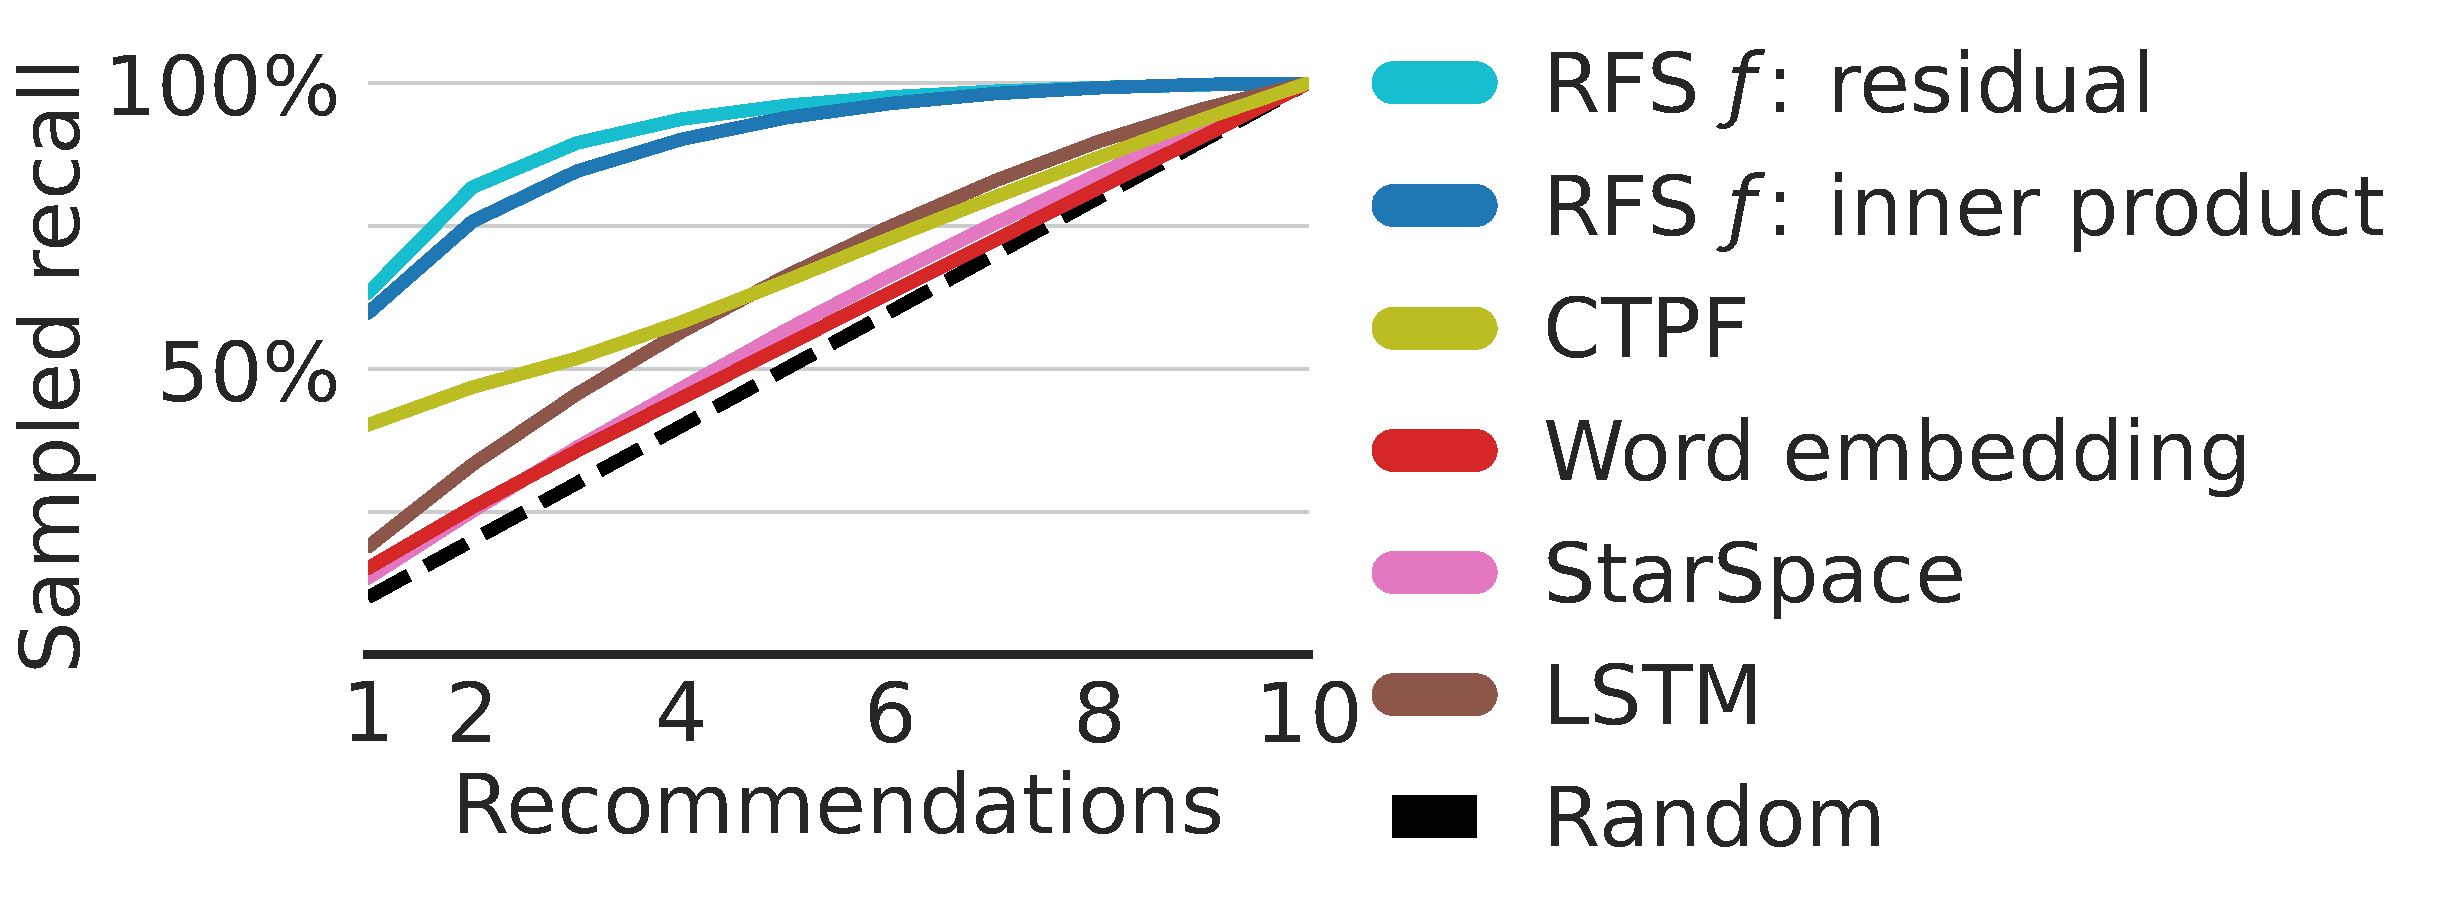
\includegraphics[width=0.7\linewidth]{ch-rfs/fig/meal-recall}
  \caption[\textsc{rfs} results on meal recommendation]{
  \textbf{\acrlong{rfs} models outperform competitors in meal
 recommendation in terms of sampled recall computed using \Cref{eq:sampled-recall}. Comparison models are described in \Cref{sec:models} (see \Cref{sec:appendix-empirical} for hyperparameters). The \gls{rfs} regression functions $f$ are defined in \Cref{eqn:rankfromsets,eqn:neural-network,eqn:residual} for the inner product, neural network, and residual models, respectively.}%
   % % The recommendation models
 % are trained on data from a food
    % tracking app as described in \Cref{sec:experiments_meals} and are evaluated
    % using the sampled recall metric, \Cref{eq:sampled-recall}. The inner
    % product, neural network, and residual regression functions for \acrlong{rfs}
    % are in \Cref{eqn:rankfromsets,eqn:neural-network,eqn:residual}
    }
  \label{fig:meal-recall}
  % \vspace{-0.5cm}
\end{figure}